\documentclass{beamer}

\usepackage[utf8]{inputenc}
%\usepackage{amsfonts,amsmath,amssymb,amsthm,booktabs,color,enumitem,graphicx}
\graphicspath{{presentation-images/}}


%Information to be included in the title page:
\title{Konvolutionaaliset neuroverkot}
\author{Teemu Sarapisto}
\institute{Helsingin Yliopisto}
\date{2018}



\begin{document}

\frame{\titlepage}

\begin{frame}
    \frametitle{Sisällys}
    - Historiaa

    - Neuroni

    - Neuroverkon rakenne

    - Neuroverkkojen harjoittaminen

    - Gradienttimenetelmä

    - (Back-propagation)

    - Konvoluutio

    - Konvolutionaalisten neuroverkkojen rakenne

    - Esimerkki konvoluutionaalisten neuroverkkojen soveltamisesta
\end{frame}

\begin{frame}
    \frametitle{Historiaa 1/5}
    Ensimmäinen neuroni McCulloch-Pitts -neuroni 1940-luvulla

    Ei vapaita parametrejä, koko systeemi suunniteltava etukäteen valmiiksi (ei opetusta)
\end{frame}

\begin{frame}
    \frametitle{Historiaa 2/5}
    Perseptroni kehitettiin 1950-luvulla

    \begin{figure}[h]
        \label{pic:perceptron}
        \centering
        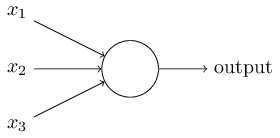
\includegraphics[scale=0.5]{perceptron}
        \caption{Perseptronin syötteet ja ulostulot}
    \end{figure}

    Perseptronin syötteet ja ulostulot ovat binäärisiä

\end{frame}

\begin{frame}
    \frametitle{Historiaa 3/5}
    1986 keksittiin soveltaa takaisinvirtausalgoritmia (back-propagation) monikerroksisten
    neuroverkkojen harjoittamiseen
\end{frame}

\begin{frame}
    \frametitle{Historiaa 4/5}
    2006 Geoffrey Hinton osoitti että verkkoja harjoitettaessa yksi taso kerrallaan
    harjoitusta saatiin tehtyä huomattavasti tehokkaammin.

    Verkkoihin aloitettiin lisäämään enemmän piilokerroksia, ja ilmiötä
    aloitettiin kuvaamaan termillä syväoppiminen (deep learning).
\end{frame}

\begin{frame}
    \frametitle{Historiaa 5/5}
    * 2012 ImageNet Large Scale Visual Recognition Challengen (ILSVRC) voitti ensimmäistä
    kertaa konvolutionaalinen neuroverkko, vieläpä huomattavalla etumatkalla toiseen sijaan.

    * Vuoden 2012 jälkeen kilpailun on joka vuosi voittanut konvolutionaalinen neuroverkko,
    tunnistamisprosentin kasvaessa vuosi vuodelta. Nykyään neuroverkot pärjäävät kyseisessä
    kilpailussa ihmistä paremmin.
\end{frame}

\begin{frame}
    \frametitle{Keinotekoisen neuronin rakenne}
    \begin{figure}[h]
        \label{pic:neuron}
        \centering
        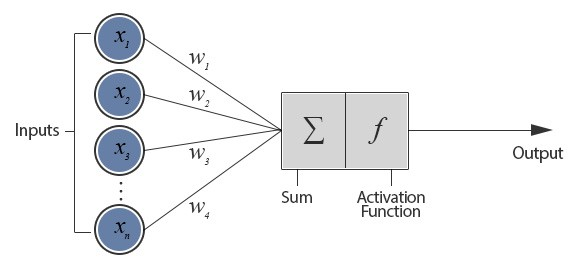
\includegraphics[scale=0.5]{artificial_neuron}
                \caption{https://medium.com/technologymadeeasy/for-dummies-the-introduction-to-neural-networks-we-all-need-c50f6012d5eb}
    \end{figure}
\end{frame}

\begin{frame}
    \frametitle{Neuroverkkojen rakenne}
    \begin{figure}[h]
        \label{pic:neural_net}
        \centering
        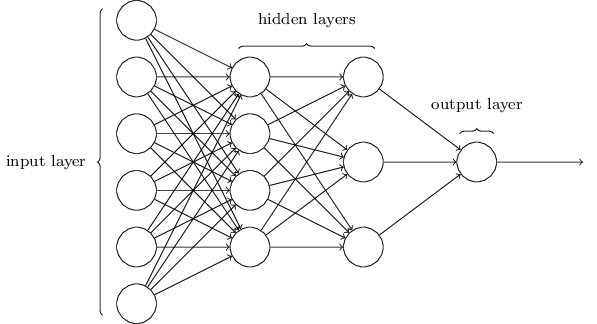
\includegraphics[scale=0.5]{basic-neuralnet}
            \caption{kuva: http://neuralnetworksanddeeplearning.com/}
    \end{figure}
\end{frame}

\begin{frame}
    \frametitle{Neuroverkkojen harjoittaminen}
    Neuroverkkojen todistettu olevan universaaleja approksimaattoreita.

    Neuroverkkojen voidaan ajatella yrittävän approksimoida jotakin funktiota.

    Neuroverkkojen harjoittaminen perustuu virheen minimointiiin tätä approksimaatiota tehtäessä.
\end{frame}

\begin{frame}
    \frametitle{Virhefunktio}

    Virhefunktiolla voidaan mitata kuinka kaukana neuroverkon tekemät approksimaatiot ovat
    todellisista funktion arvoista.

\end{frame}

\begin{frame}
    \frametitle{Virhefunktio}
    Esimerkiksi neliöllinen virhefunktio

    $$E(x) = \frac{1}{2} \sum_{i=1}^{N} \| y(x_i)-a(x_i) \|^2$$
  jossa $y(x_i)$ on neuroverkon tulos syötteellä $x_i$, $a(x_i)$ on harjoitusdatan $i$:s yksikkö, ja $N$ syötteiden määrä.

\end{frame}

\begin{frame}
    \frametitle{Virhefunktion minimointi}
    Virhettä minimoidaan laskemalla verkon painojen derivaatat virhefunktion suhteen,
    ja soveltamalla niihin gradienttimenetelmää.

    Derivaatat saadaan selville takaisinvirtausalgoritmilla (back-propagation)
\end{frame}

\begin{frame}
    \frametitle{Gradienttimenetelmä}
    \begin{figure}[h]
        \label{pic:gradient_descent}
        \centering
        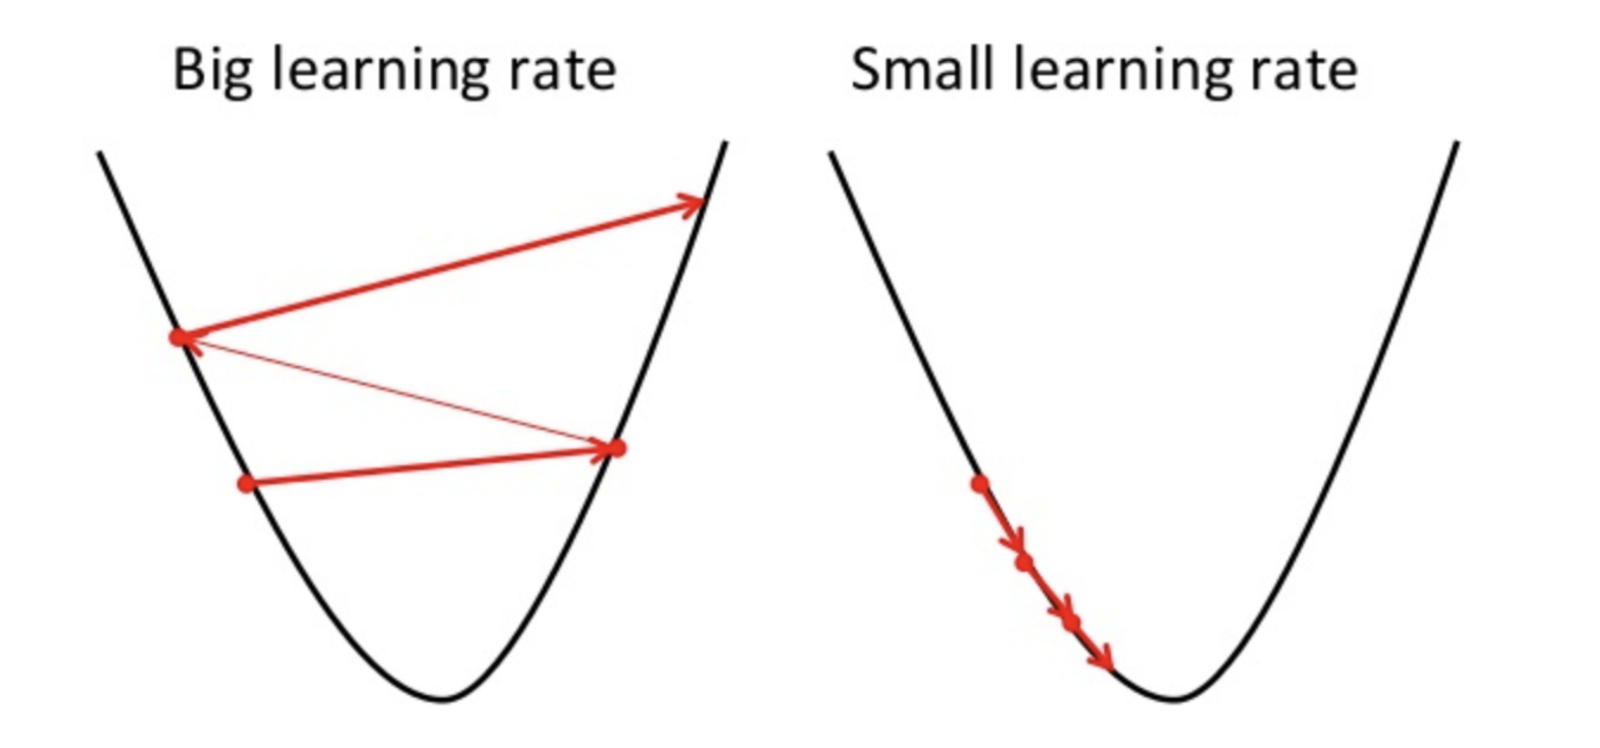
\includegraphics[scale=0.15]{gradient_descent}
        \caption{https://towardsdatascience.com/gradient-descent-in-a-nutshell-eaf8c18212f0}
    \end{figure}

    Funktion gradientti kertoo mihin suuntaan funktion arvo laskee nopeimmin, joten siirryttäessä
    askel askeleelta tähän suuntaan, lähestytään funktion lokaalia minimiä.

\end{frame}

\begin{frame}
    \frametitle{Takaisinvirtausalgoritmi}
    Neuroverkon voidaan ajatella olevan yhdistetty funktio sen neuroneiden funktioista.

    Derivaatan ketjusääntöä hyödyntämällä voidaan kulkea neuroverkkoa taaksepäin selvittäen
    painojen derivaatat virhefunktion suhteen.
\end{frame}

\begin{frame}
    \frametitle{Ylisovitus (overfitting)}
    Suorittamalla virhefunktion minimointia harjoitusdatalle liian pitkälle,
    neuroverkko saa harjoitusdatalle pieniä tuloksia virhefunktiosta, mutta esitettäessä sille
    uutta dataa se tekee suuria virheitä.

    Tällöin verkko on ylisovittunut, eli harjoitusdatan yleistäminen on epäonnistunut.
\end{frame}

\begin{frame}
    \frametitle{Konvolutionaaliset neuroverkot}
    Eroavat muista keinotekoisista neuroverkoista ensisijaisesti konvoluutio- ja kokoamiskerroksien
    kautta.
\end{frame}

\begin{frame}
    \frametitle{Konvoluutio}
    \begin{figure}[h]
        \label{pic:convolution}
        \centering
        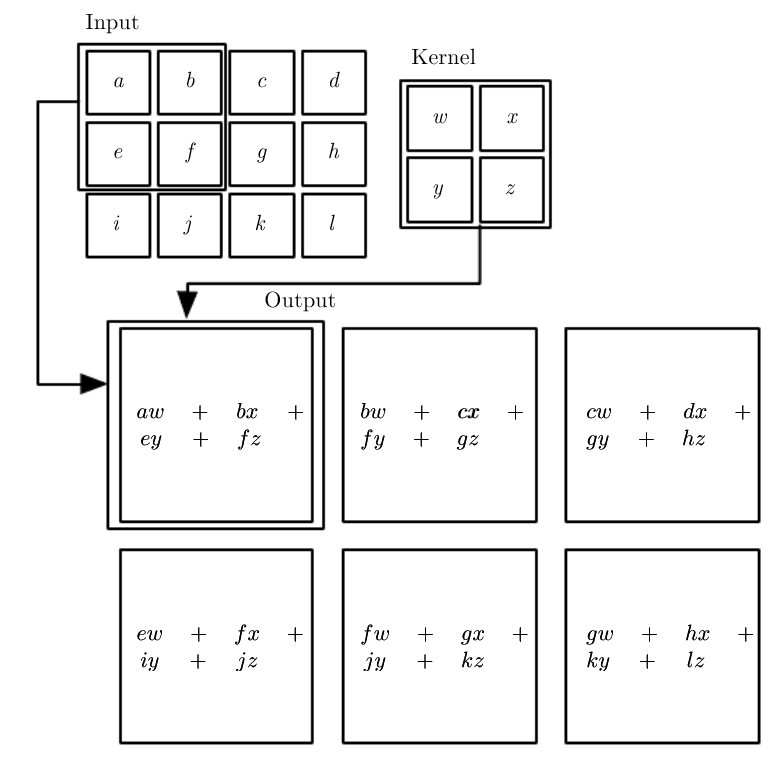
\includegraphics[scale=0.28]{convolution}
        \caption{http://www.deeplearningbook.org}

    \end{figure}
\end{frame}

\begin{frame}
    \frametitle{Konvoluutio intuitiivisesti}
    Liukuva ikkuna joka rajoittaa neuronin syötteet vain osaan syötekerroksen ulostuloista, poiketen
    normaaleista täysin yhdistetyistä kerroksista.

    Tämä auttaa neuroneita hyödyntämään esimerkiksi kuvissa ilmenevää paikallisuutta:
    pikselien etäisyys toisistaan korreloi vahvasti sen kanssa, liittyykö niiden sisältö toisiinsa.
\end{frame}


\begin{frame}
    \frametitle{Ominaisuuskartat}
    Konvoluutiokerrroksia on yleensä useita rinnakkain, ja kerroksen neuroneilla painot ovat yhteisiä

    Yhteiset painot mahdollistavat sen, että neuronit oppivat tunnistamaan sijainnista riippumattomia
    ominaisuuksia kuvasta, ja yksittäinen neuroni kerroksessa kertoo löytyykö sen ikkunasta kyseistä
    ominaisuutta.
\end{frame}

\begin{frame}
    \frametitle{Ominaisuuskartat}
    Yhdistetään hommelit
\end{frame}

\begin{frame}
    \frametitle{Kokoaminen}
    Yhdistetään hommelit
\end{frame}

\begin{frame}
    \frametitle{Kiitos t. kiitos}
    Yhdistetään hommelit
\end{frame}

\end{document}